
% Copyright (c) 2015 - 2020 Mario Mlačak, mmlacak@gmail.com
% Published as Public Domain work, under CC0 1.0 Universal Public Domain Dedication. See LICENSING, COPYING files for details.

% Conquest of Tlalocan chapter ========================================
\chapter*{Conquest of Tlalocan}
\addcontentsline{toc}{chapter}{Conquest of Tlalocan}
\label{ch:Conquest of Tlalocan}

\begin{flushright}
\parbox{0.78\textwidth}{
\emph{The greatest difficulty with the world is not its ability to produce, but the unwillingness to share. \newline
\hspace*{\fill}{\textperiodcentered \textperiodcentered \textperiodcentered \hspace*{0.2em} Roy L. Smith} } }
\end{flushright}

\noindent
Conquest of Tlalocan is chess variant which is played on 24 x 24 board,
with bright red and cyan fields, and dark red and light green pieces.
Star colors are bright red and bright blue.
A new piece is introduced, Shaman.

\clearpage % ..........................................................
% Shaman **************************************************************

\section*{Shaman}
\addcontentsline{toc}{section}{Shaman}
\label{sec:Conquest of Tlalocan/Shaman}

\vspace*{-0.7\baselineskip}
\noindent
\begin{wrapfigure}[10]{l}{0.4\textwidth}
\centering
\includegraphics[width=0.4\textwidth, keepaspectratio=true]{pieces/16_shaman.png}
\vspace*{-1.4\baselineskip}
\caption{Shaman}
\label{fig:16_shaman}
\end{wrapfigure}
Shaman moves like sort-of cross between Knight and long-jump Unicorn,
where one figure provides step-fields, and the other capture-fields.

For light Shaman, step-fields are provided by the Knight, while capture-fields
are provided by long-range Unicorn. For dark Shaman, it's the opposite.

Shaman can continue its jumpy movement in chosen direction; over step-fields
if they're empty, over capture-fields as long as it's capturing opponent's
pieces. Shaman can't change direction once started moving.

\noindent
\begin{wrapfigure}[10]{l}{0.4\textwidth}
\centering
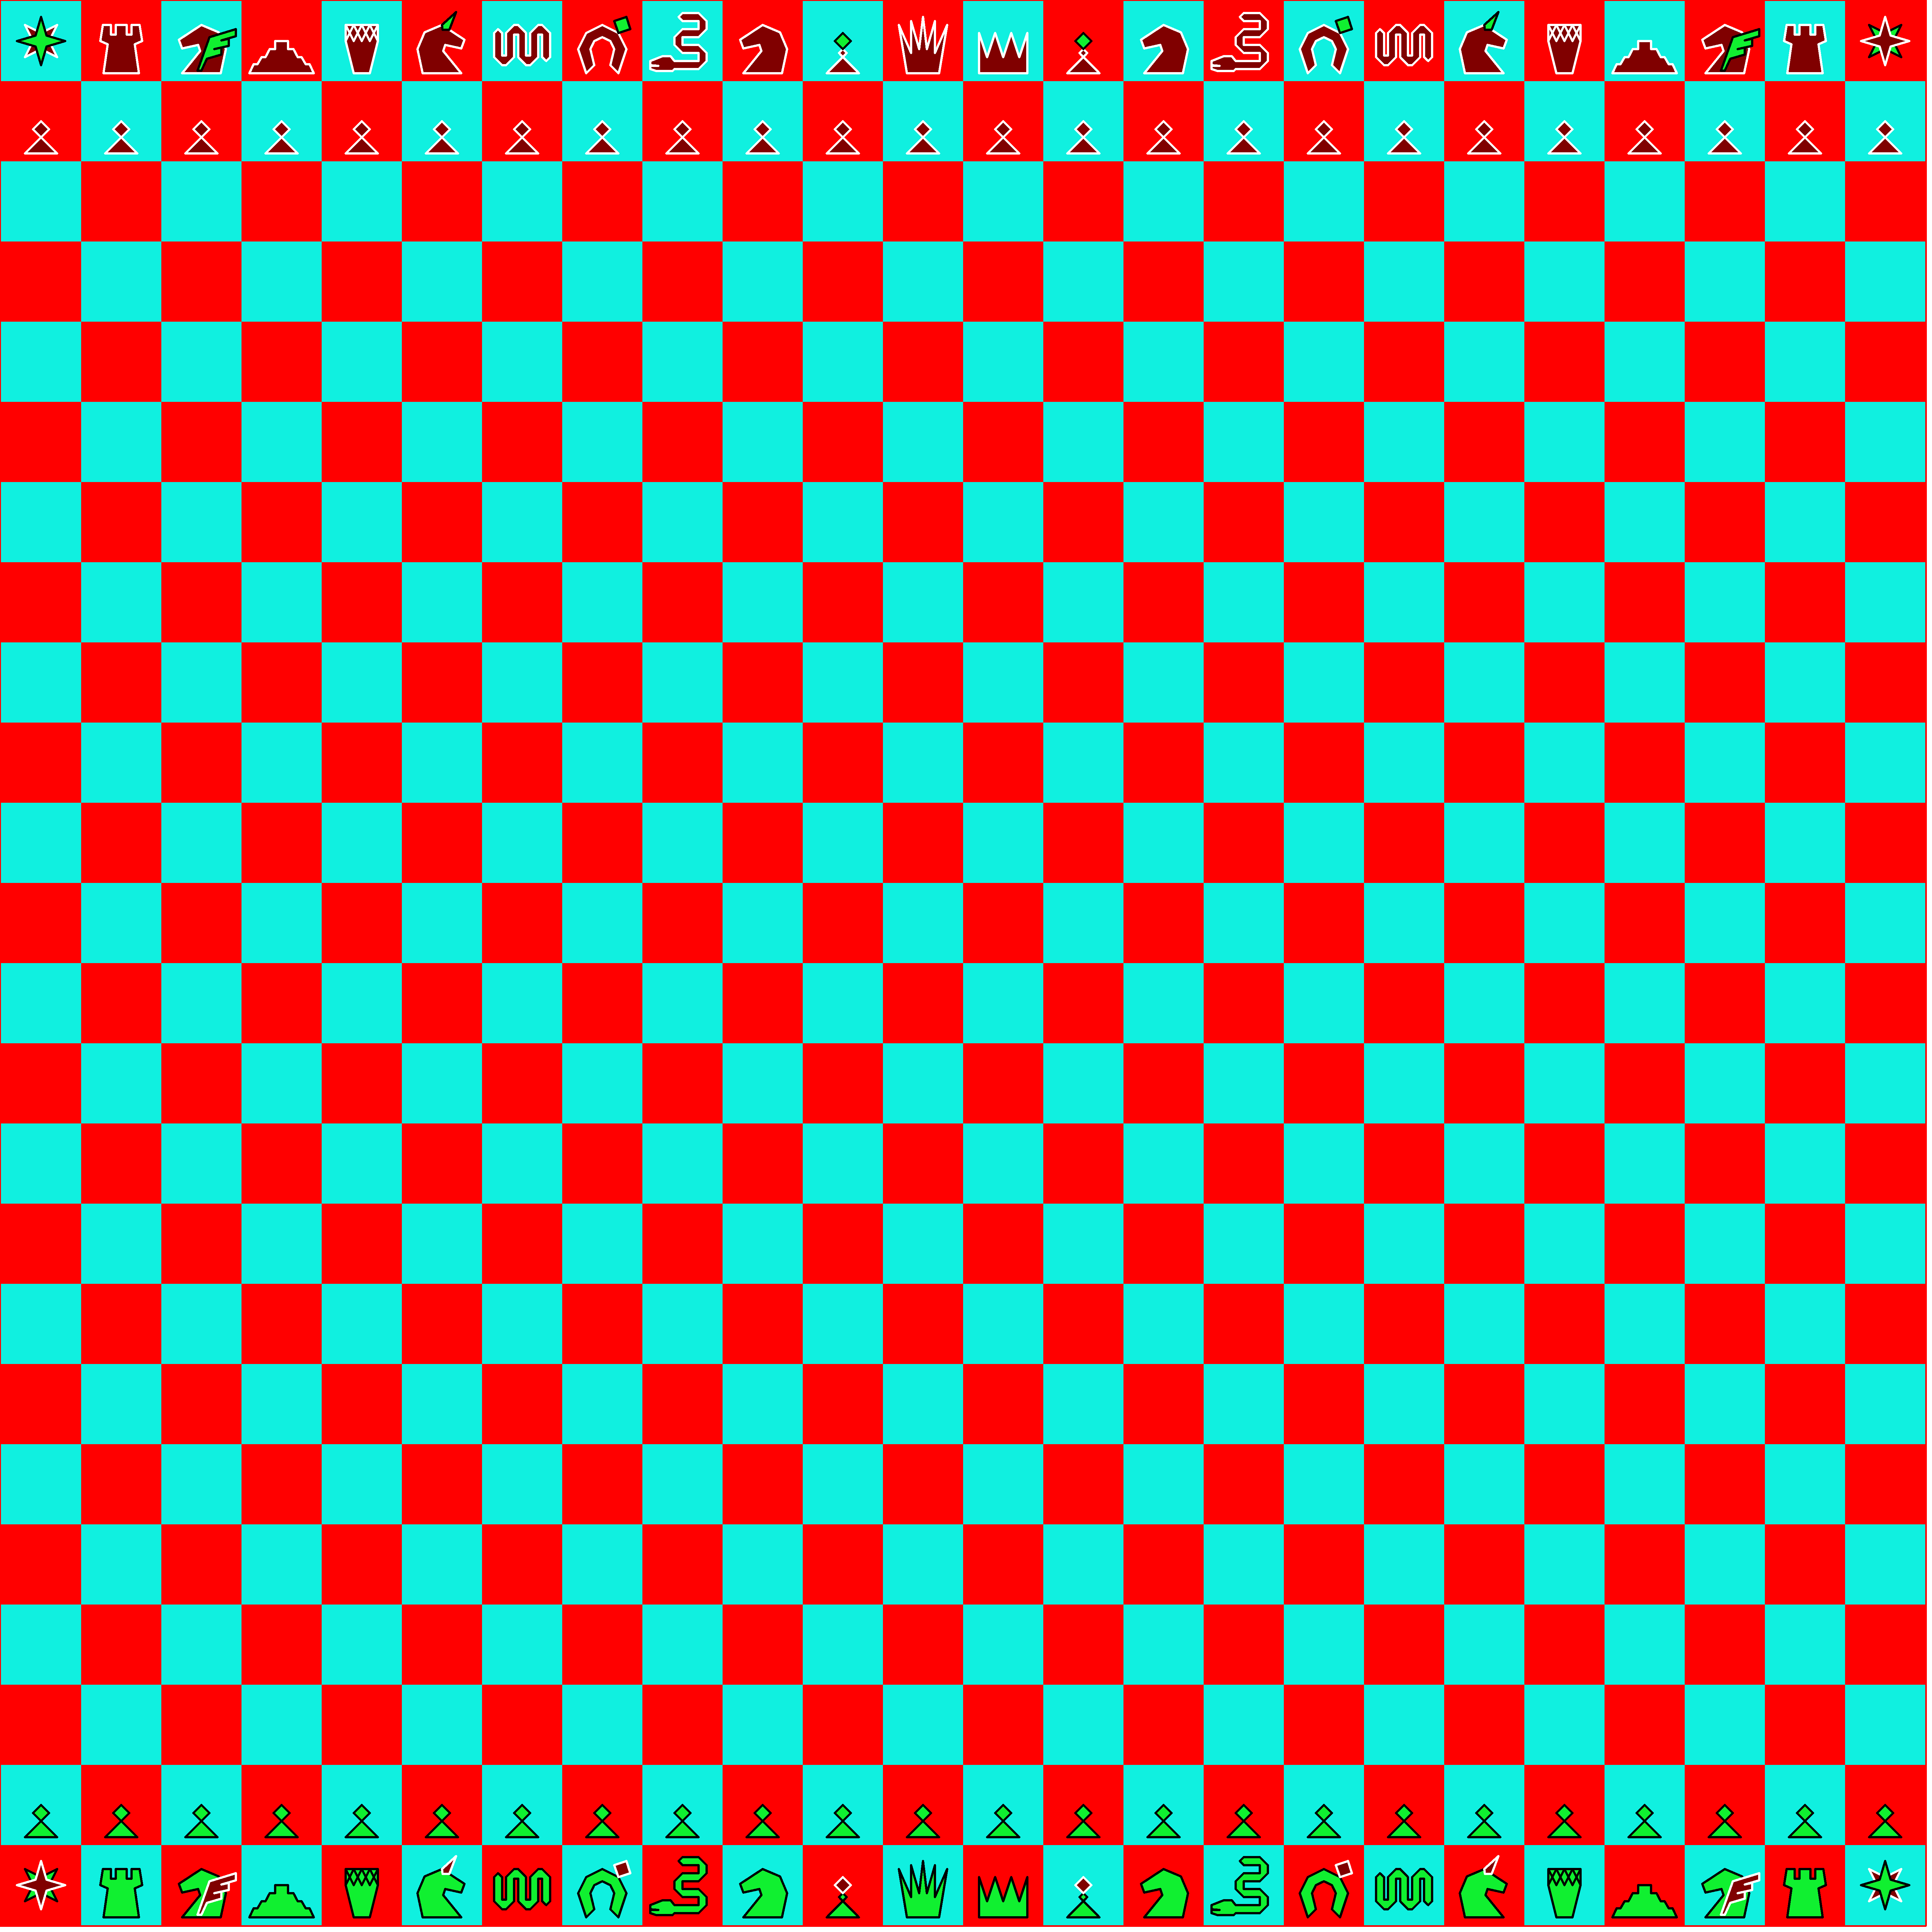
\includegraphics[width=0.4\textwidth, keepaspectratio=true]{pieces/star/18_conquest_of_tlalocan.png}
\vspace*{-1.4\baselineskip}
\caption{Star}
\label{fig:star/18_conquest_of_tlalocan}
\end{wrapfigure}
Shaman is divergent; any own piece (and opponent's Shaman) can change direction
when they encounter Shaman, after which they use remaining momentum to move.

Shaman can also take on a trance-journey, and displace or capture multiple
pieces.

\noindent
For this variant examples are rendered in B\&W to improve legibility.

\clearpage % ..........................................................
% Movement ------------------------------------------------------------

\subsection*{Movement}
\addcontentsline{toc}{subsection}{Movement}
\label{sec:Conquest of Tlalocan/Shaman/Movement}

\vspace*{-1.4\baselineskip}
\noindent
\begin{figure}[!h]
\includegraphics[width=1.0\textwidth, keepaspectratio=true]{examples/18_cot/scn_cot_001_shaman_movement.png}
\vspace*{-1.4\baselineskip}
\caption{Shaman's movement}
\label{fig:scn_cot_001_shaman_movement}
\end{figure}

\vspace*{-0.4\baselineskip}
Shaman has its step-fields (here, green) separated from capture-fields (blue). For
light Shaman, step-fields are the same as Knight's, while capture-fields are accessed
after long jump, \hyperref[fig:scn_aoa_02_unicorn_opposite_color]{similar to Unicorn's}.
For dark Shamans, it's the opposite; step-fields are available after long jump, while
capture fields are the same as Knight's. Unlike Unicorn, movement of Shaman does not
depend on color of field on which it stands, only on color of the piece itself.

\clearpage % ..........................................................

\subsubsection*{Light Shaman's step-ply}
\addcontentsline{toc}{subsubsection}{Light Shaman's step-ply}
\label{sec:Conquest of Tlalocan/Shaman/Movement/Light Shaman's step-ply}

\vspace*{-1.4\baselineskip}
\noindent
\begin{figure}[!h]
\includegraphics[width=1.0\textwidth, keepaspectratio=true]{examples/18_cot/scn_cot_002_light_shaman_step_ply.png}
\vspace*{-1.4\baselineskip}
\caption{Light Shaman's step-ply}
\label{fig:scn_cot_002_light_shaman_step_ply}
\end{figure}

\vspace*{-0.4\baselineskip}
Light Shaman can choose any step-field for its initial direction; once chosen, Shaman
has to follow it for the remainder of a ply. Direction of a ply cannot be changed,
neither in other step- nor any capture-field (red arrows in the example above).

Wave on a step-field can be activated, and would move as Shaman does.
\hyperref[fig:scn_mv_07_wave_is_transparent]{Wave is transparent} to Shaman, and
so does not prevent Shaman from continuing its ply.

\noindent
\begin{wrapfigure}[8]{l}{0.4\textwidth}
\centering
\includegraphics[width=0.4\textwidth, keepaspectratio=true]{examples/18_cot/scn_cot_003_light_shaman_step_ply_no_capture.png}
\vspace*{-1.4\baselineskip}
\caption{No capture}
\label{fig:scn_cot_003_light_shaman_step_ply_no_capture}
\end{wrapfigure}
Shaman can't capture opponent's piece on a step-field, nor activate Pyramid (in
the example above). Most pieces are not transparent to Shaman, so when they're
encountered on its step-fields, Shaman is prevented from moving any further.

\clearpage % ..........................................................

\subsubsection*{Light Shaman's capture-ply}
\addcontentsline{toc}{subsubsection}{Light Shaman's capture-ply}
\label{sec:Conquest of Tlalocan/Shaman/Movement/Light Shaman's capture-ply}

\vspace*{-1.4\baselineskip}
\noindent
\begin{figure}[!h]
\includegraphics[width=1.0\textwidth, keepaspectratio=true]{examples/18_cot/scn_cot_004_light_shaman_capture_ply.png}
\vspace*{-1.4\baselineskip}
\caption{Light Shaman's capture-ply}
\label{fig:scn_cot_004_light_shaman_capture_ply}
\end{figure}

\vspace*{-0.4\baselineskip}
Shaman can capture opponent's pieces only on its capture-fields. After initial capture,
Shaman can continue capturing in the same ply, and in the same direction, as long as
there are opponent's pieces to capture. Once capturing, Shaman cannot change direction
of a ply into any step- or other capture-field, even if opponent's piece is placed
there (above, red arrows). Empty capture-fields cannot be overstepped, any piece at
a distant capture-field is out of reach.

\noindent
\begin{wrapfigure}[6]{l}{0.4\textwidth}
\centering
\includegraphics[width=0.391666667\textwidth, keepaspectratio=true]{examples/18_cot/scn_cot_005_light_shaman_capture_ply_passives.png}
\vspace*{-1.4\baselineskip}
\caption{Activation}
\label{fig:scn_cot_005_light_shaman_capture_ply_passives}
\end{wrapfigure}
Capture-ply can end with Shaman activating either Wave or Pyramid on its capture-field.
Activation can be done as a first action in a ply, without any opponent's pieces being
captured.

Note that in the previous example, even though Wave is transparent to Shaman, Pyramid
is out of reach because transparency is lack of interaction, so it's effectively the
same as empty capture-field, which cannot be overstepped.

\clearpage % ..........................................................

\subsubsection*{Dark Shaman's step-ply}
\addcontentsline{toc}{subsubsection}{Dark Shaman's step-ply}
\label{sec:Conquest of Tlalocan/Shaman/Movement/Dark Shaman's step-ply}

\vspace*{-1.4\baselineskip}
\noindent
\begin{figure}[!h]
\includegraphics[width=1.0\textwidth, keepaspectratio=true]{examples/18_cot/scn_cot_006_dark_shaman_step_ply.png}
\vspace*{-1.4\baselineskip}
\caption{Dark Shaman's step-ply}
\label{fig:scn_cot_006_dark_shaman_step_ply}
\end{figure}

\vspace*{-0.4\baselineskip}
Dark Shaman's stepping ply is the same as
\hyperref[fig:scn_cot_002_light_shaman_step_ply]{light Shaman's}, except it uses
Unicorn's long jumps as steps.

\vspace*{-1.4\baselineskip}
\subsubsection*{Dark Shaman's capture-ply}
\addcontentsline{toc}{subsubsection}{Dark Shaman's capture-ply}
\label{sec:Conquest of Tlalocan/Shaman/Movement/Dark Shaman's capture-ply}

\vspace*{-1.4\baselineskip}
\noindent
\begin{figure}[!h]
\includegraphics[width=1.0\textwidth, keepaspectratio=true]{examples/18_cot/scn_cot_008_dark_shaman_capture_ply.png}
\vspace*{-1.4\baselineskip}
\caption{Dark Shaman's capture-ply}
\label{fig:scn_cot_008_dark_shaman_capture_ply}
\end{figure}

\vspace*{-0.4\baselineskip}
Dark Shaman's capturing ply is the same as
\hyperref[fig:scn_cot_004_light_shaman_capture_ply]{light Shaman's}, except it uses
Knight's (short) jumps as capture-steps.

\clearpage % ..........................................................

\subsubsection*{Activating Wave}
\addcontentsline{toc}{subsubsection}{Activating Wave}
\label{sec:Conquest of Tlalocan/Shaman/Movement/Activating Wave}

\vspace*{-0.7\baselineskip}
\noindent
\begin{wrapfigure}[9]{l}{0.4\textwidth}
\centering
\includegraphics[width=0.391666667\textwidth, keepaspectratio=true]{examples/18_cot/scn_cot_010_activating_wave_step_field.png}
\vspace*{-1.4\baselineskip}
\caption{Activating Wave on step-fields}
\label{fig:scn_cot_010_activating_wave_step_field}
\end{wrapfigure}
Activated Wave moves the same as activating Shaman, i.e. using the same kind of
a step (either ordinary step, or capture-step) Shaman had in the moment of activation. \newline
\indent
On the left, Wave is about to be activated by light Shaman on its step-field, so
Wave would move using Knight's (short) jump as a step.

\noindent
\begin{wrapfigure}[13]{l}{0.4\textwidth}
\centering
\includegraphics[width=0.391666667\textwidth, keepaspectratio=true]{examples/18_cot/scn_cot_011_activating_wave_capture_field.png}
\vspace*{-1.4\baselineskip}
\caption{Activating Wave on capture-fields}
\label{fig:scn_cot_011_activating_wave_capture_field}
\end{wrapfigure}
The same as activating Shaman, activated Wave cannot change direction in the middle
of its ply, regardless if activated on a step- or a capture-field. \newline
\indent
Here, Wave is about to be activated by light Shaman on its capture-field, so Wave
would move using Unicorn's (long) jump as a step.

Note, Wave activated by Shaman on its capture-field can move over empty fields,
even though activating Shaman itself cannot. Activated Wave also doesn't have to
perform an action (e.g. activate a piece) on every field it visits, even though
activating Shaman itself has to e.g. capture a piece. \newline
\indent
Above, activated light Wave can pass-by Pyramid (since it's transparent to Wave),
skip over an empty field, and e.g. activate light Knight on a distant field.

\clearpage % ..........................................................

% \vspace*{0.7\baselineskip} % 6.7
\TODO :: back-link to sec:Miranda's veil/Wave/Movement/Activated by Pawn/TODO

\clearpage % ..........................................................

\subsubsection*{Shaman is semi-transparent}
\addcontentsline{toc}{subsubsection}{Shaman is semi-transparent}
\label{sec:Conquest of Tlalocan/Shaman/Movement/Shaman is semi-transparent}

\vspace*{-0.7\baselineskip}
\noindent
\begin{wrapfigure}[6]{l}{0.4\textwidth}
\centering
\includegraphics[width=0.391666667\textwidth, keepaspectratio=true]{examples/18_cot/scn_cot_012_shaman_transparent_to_own_pieces.png}
\vspace*{-1.4\baselineskip}
\caption{Transparent to own pieces}
\label{fig:scn_cot_012_shaman_transparent_to_own_pieces}
\end{wrapfigure}
Shaman \hyperref[fig:scn_mv_07_wave_is_transparent]{is transparent} to all own pieces. \newline
\indent
Here, light Bishop cannot activate own Shaman, but it can continue its movement
past light Shaman.

\vspace*{2.7\baselineskip}
\noindent
\begin{wrapfigure}[6]{l}{0.4\textwidth}
\centering
\includegraphics[width=0.391666667\textwidth, keepaspectratio=true]{examples/18_cot/scn_cot_013_shaman_not_transparent_to_opponents_pieces.png}
\vspace*{-1.4\baselineskip}
\caption{Opaque to opponent's pieces}
\label{fig:scn_cot_013_shaman_not_transparent_to_opponents_pieces}
\end{wrapfigure}
Shaman is opaque (i.e. is not transparent) to all opponent's pieces, except Shaman. \newline
\indent
Here, dark Bishop can capture opponent's Shaman, but it cannot move past light Shaman.

\vspace*{2.7\baselineskip}
\noindent
\begin{wrapfigure}[6]{l}{0.4\textwidth}
\centering
\includegraphics[width=0.391666667\textwidth, keepaspectratio=true]{examples/18_cot/scn_cot_014_shaman_transparent_to_opponents_shaman.png}
\vspace*{-1.4\baselineskip}
\caption{Transparent to opponent's Shaman}
\label{fig:scn_cot_014_shaman_transparent_to_opponents_shaman}
\end{wrapfigure}
Shaman is also transparent to opponent's Shaman. \newline
\indent
Here, dark Shaman can either capture opponent's Shaman, or it can continue its movement
past light Shaman.

\vspace*{2.7\baselineskip}
\TODO \newline
1. fix example above \newline
2. activated piece must have momentum to pass-through transparent Shaman \newline
3. link 2. from sec:Conquest of Tlalocan/Divergence/... if activated

\clearpage % ..........................................................

\subsubsection*{Unicorn is transparent to Shamans}
\addcontentsline{toc}{subsubsection}{Unicorn is transparent to Shamans}
\label{sec:Conquest of Tlalocan/Shaman/Movement/Unicorn is transparent to Shamans}

\vspace*{-0.7\baselineskip}
\noindent
\begin{wrapfigure}[6]{l}{0.4\textwidth}
\centering
\includegraphics[width=0.391666667\textwidth, keepaspectratio=true]{examples/18_cot/scn_cot_015_unicorn_is_transparent_to_own_shaman.png}
\vspace*{-1.4\baselineskip}
\caption{Transparent to own Shaman}
\label{fig:scn_cot_015_unicorn_is_transparent_to_own_shaman}
\end{wrapfigure}
Unicorn \hyperref[fig:scn_mv_07_wave_is_transparent]{is transparent} only to Shamans,
both own, and opponent's. \newline
\indent
Here, light Shaman cannot activate own Unicorn, but it can move past light Unicorn.

% \vspace*{-0.7\baselineskip}
\noindent
\begin{wrapfigure}[4]{l}{0.4\textwidth}
\centering
\includegraphics[width=0.391666667\textwidth, keepaspectratio=true]{examples/18_cot/scn_cot_016_unicorn_is_transparent_to_opponents_shaman.png}
\vspace*{-1.4\baselineskip}
\caption{Transparent to opponent's Shaman}
\label{fig:scn_cot_016_unicorn_is_transparent_to_opponents_shaman}
\end{wrapfigure}
Here, dark Shaman can either capture opponent's Unicorn, or it can continue its movement
past light Unicorn.

\vspace*{1.7\baselineskip}
\noindent
\begin{wrapfigure}[6]{l}{0.4\textwidth}
\centering
\includegraphics[width=0.391666667\textwidth, keepaspectratio=true]{examples/18_cot/scn_cot_017_unicorn_is_opaque_to_own_pieces.png}
\vspace*{-1.4\baselineskip}
\caption{Opaque to own pieces}
\label{fig:scn_cot_017_unicorn_is_opaque_to_own_pieces}
\end{wrapfigure}
Unicorn is opaque (not transparent) to all other pieces, own and opponent's. \newline
\indent
Here, light Pegasus cannot activate own Unicorn, and is blocked from moving any further.

\vspace*{.7\baselineskip}
\noindent
\begin{wrapfigure}[3]{l}{0.4\textwidth}
\centering
\includegraphics[width=0.391666667\textwidth, keepaspectratio=true]{examples/18_cot/scn_cot_018_unicorn_is_opaque_to_opponents_pieces.png}
\vspace*{-1.4\baselineskip}
\caption{Opaque to opponent's pieces}
\label{fig:scn_cot_018_unicorn_is_opaque_to_opponents_pieces}
\end{wrapfigure}
Here, dark Pegasus can capture opponent's Unicorn, but it cannot move past light Unicorn.

\clearpage % ..........................................................

\subsubsection*{Teleporting Shaman}
\addcontentsline{toc}{subsubsection}{Teleporting Shaman}
\label{sec:Conquest of Tlalocan/Shaman/Movement/Teleporting Shaman}

\vspace*{-1.4\baselineskip}
\noindent
\begin{figure}[!h]
\includegraphics[width=1.0\textwidth, keepaspectratio=true]{examples/18_cot/scn_cot_019_teleport_shaman_all.png}
\vspace*{-1.4\baselineskip}
\caption{Teleporting Shaman}
\label{fig:scn_cot_019_teleport_shaman_all}
\end{figure}

\vspace*{-0.4\baselineskip}
Image above have three examples in parallel; each starting with one of light
Shamans A, B, and C.

Shaman can reach a Star and start teleporting after capturing spree (Shaman A),
by diving directly into a Star on a capture-field (B), or after a non-capturing
ply (C). In all cases, Shaman would reappear on an empty portal-field, next to a
Star in opposite color (here, any of fields 1 -- 6).

\clearpage % ..........................................................

\subsubsection*{Teleporting Pawn}
\addcontentsline{toc}{subsubsection}{Teleporting Pawn}
\label{sec:Conquest of Tlalocan/Shaman/Movement/Teleporting Pawn}

\vspace*{-1.4\baselineskip}
\noindent
\begin{figure}[!h]
\includegraphics[width=1.0\textwidth, keepaspectratio=true]{examples/18_cot/scn_cot_020_teleport_pawn_init.png}
\vspace*{-1.4\baselineskip}
\caption{Teleporting Pawn}
\label{fig:scn_cot_020_teleport_pawn_init}
\end{figure}

\vspace*{-0.4\baselineskip}
In this variant
\hyperref[sec:Conquest of Tlalocan/Promotion]{promotion is immediate}, so Pawns
cannot be tagged for promotion.
Pawn teleported to opponent's \hyperref[sec:Terms/Figure row]{figure row} (here,
field 1) has to be promoted immediately. Pawn teleported to opponent's Pawn row
(fields 2, 3) won't be tagged for promotion. \newline
\indent
Pawn teleported onto own side of a board (portal-fields 4, 5, 6) does not gain
opportunity to rush on initial move; the same as in
\hyperref[fig:scn_n_12_teleport_pawns_step_1]{previous variant, Nineteen}.

% ------------------------------------------------------------ Movement
% ************************************************************** Shaman
\clearpage % ..........................................................
% Divergence **********************************************************

\section*{Divergence}
\addcontentsline{toc}{section}{Divergence}
\label{sec:Conquest of Tlalocan/Divergence}

\vspace*{-1.4\baselineskip}
\noindent
\begin{figure}[!h]
\includegraphics[width=1.0\textwidth, keepaspectratio=true]{examples/18_cot/scn_cot_030_own_shaman_is_divergent_init.png}
\vspace*{-1.3\baselineskip}
\caption{Own Shaman is divergent}
\label{fig:scn_cot_030_own_shaman_is_divergent_init}
\end{figure}

\vspace*{-0.5\baselineskip}
Piece, when encounters own Shaman, can continue its movement, and changes direction
to any available, as if starting a new ply from a position of encountered Shaman.
Direction change is divergence, after which piece is limited by momentum it had when
own Shaman was encountered. \newline
\indent
Here, light Queen can diverge only from own, light Shaman; but not from opponent's,
dark Shaman.

\clearpage % ..........................................................

\vspace*{-2.1\baselineskip}
\noindent
\begin{figure}[!h]
\includegraphics[width=1.0\textwidth, keepaspectratio=true]{examples/18_cot/scn_cot_031_own_shaman_is_divergent_end.png}
\vspace*{-1.3\baselineskip}
\caption{Diverging Queen}
\label{fig:scn_cot_031_own_shaman_is_divergent_end}
\end{figure}

\vspace*{-0.4\baselineskip}
Here, light Queen (now "in the air") has reached own Shaman, and can choose a new
direction of movement independently of previous choice. Note that light Queen can
move for only 5 fields, since diverging piece is limited by momentum it had when
own Shaman was reached.

The only piece in a move, just like piece starting a cascade,
\hyperref[fig:scn_mv_46_static_move_is_illegal_init]{cannot end its move on a starting field}.
So, in this example, starting field Q is illegal destination for light Queen.

\clearpage % ..........................................................
% Diverging activated piece -------------------------------------------

\subsection*{Diverging activated piece}
\addcontentsline{toc}{subsection}{Diverging activated piece}
\label{sec:Conquest of Tlalocan/Divergence/Diverging activated piece}

\vspace*{-1.4\baselineskip}
\noindent
\begin{figure}[!h]
\includegraphics[width=1.0\textwidth, keepaspectratio=true]{examples/18_cot/scn_cot_032_diverging_activated_piece_init.png}
\vspace*{-1.3\baselineskip}
\caption{Activating Rook}
\label{fig:scn_cot_032_diverging_activated_piece_init}
\end{figure}

\vspace*{-0.4\baselineskip}
Activated piece can also diverge, but it's already limited by received momentum
while going towards divergent Shaman, as it's limited after diverging.

Activated, material piece which has no momentum when own Shaman is reached cannot
diverge from it, only stop before it.

\clearpage % ..........................................................

\vspace*{-2.1\baselineskip}
\noindent
\begin{figure}[!h]
\includegraphics[width=1.0\textwidth, keepaspectratio=true]{examples/18_cot/scn_cot_033_diverging_activated_piece_end.png}
\vspace*{-1.3\baselineskip}
\caption{Diverging activated Rook}
\label{fig:scn_cot_033_diverging_activated_piece_end}
\end{figure}

\vspace*{-0.4\baselineskip}
In previous example, activated Rook couldn't diverge from Shaman B, only stop before
it is reached, since all received momentum would be spent moving towards Shaman B.

The same Rook (now "in the air") can diverge from Shaman A, with 2 remaining momentum,
i.e. difference between received momentum and amount spent moving towards Shaman A.

% ------------------------------------------- Diverging activated piece
\clearpage % ..........................................................
% Diverging Pawn ------------------------------------------------------

\subsection*{Diverging Pawn}
\addcontentsline{toc}{subsection}{Diverging Pawn}
\label{sec:Conquest of Tlalocan/Divergence/Diverging Pawn/2} % line 264

\vspace*{-1.4\baselineskip}
\noindent
\begin{figure}[!h]
\includegraphics[width=1.0\textwidth, keepaspectratio=true]{examples/18_cot/scn_cot_034_diverging_pawn_init.png}
\vspace*{-1.3\baselineskip}
\caption{Diverging Pawns start}
\label{fig:scn_cot_034_diverging_pawn_init}
\end{figure}

\vspace*{-0.5\baselineskip}
Image above and the next one have five examples presented in parallel; each with
its own, labeled Pawn. \newline
\indent
Pawn can diverge from own Shaman by making forward-, sideways-, or capture-step,
or by rushing. After divergence, steps are available as if starting a new ply;
forward- and sideways-steps if not blocked; capture-steps if opponent's piece is
placed on a Pawn's capture-field behind own, divergent Shaman.

\clearpage % ..........................................................

\vspace*{-2.1\baselineskip}
\noindent
\begin{figure}[!h]
\includegraphics[width=1.0\textwidth, keepaspectratio=true]{examples/18_cot/scn_cot_035_diverging_pawn_end.png}
\vspace*{-1.3\baselineskip}
\caption{Diverging Pawns end}
\label{fig:scn_cot_035_diverging_pawn_end}
\end{figure}

\vspace*{-0.4\baselineskip}
Image above have all five Pawns "in the air", each can choose its next direction
independently of arriving path; each from its own, divergent Shaman. \newline
\indent
Diverging Pawn is limited to only one step, regardless how much momentum it had
when own Shaman was encountered. Here, activated Pawn E can make only one step
forward, even though it had 4 momentum when light Shaman was reached. The sole
exception to this limitation is rushing Pawn (here, C), which can step forward
for more than one field.

% ------------------------------------------------------ Diverging Pawn
\clearpage % ..........................................................

\subsection*{Diverging rushing Pawn}
\addcontentsline{toc}{subsection}{Diverging rushing Pawn}
\label{sec:Conquest of Tlalocan/Divergence/Diverging rushing Pawn}

\vspace*{-1.4\baselineskip}
\noindent
\begin{figure}[!h]
\includegraphics[width=1.0\textwidth, keepaspectratio=true]{examples/18_cot/scn_cot_036_diverging_rushing_pawn.png}
\vspace*{-1.3\baselineskip}
\caption{Diverging rushing Pawn}
\label{fig:scn_cot_036_diverging_rushing_pawn}
\end{figure}

\vspace*{-0.5\baselineskip}
Image above have four examples presented in parallel; each with labeled Pawn starting
a cascade. \newline
\indent
Rushing Pawn can diverge from own Shaman (here, Pawns B, C), or it has to stop before
own Shaman is encountered (Pawn A). Rushing Pawns are limited by momentum, so
divergent Shaman closer to starting field will limit Pawn's reach (Pawn B), while
Shaman farther apart will extend it (Pawn C), compared to full extent of ordinary
rush (Pawn D).

\clearpage % ..........................................................
% Diverging Unicorn ---------------------------------------------------

\subsection*{Diverging Unicorn}
\addcontentsline{toc}{subsection}{Diverging Unicorn}
\label{sec:Conquest of Tlalocan/Divergence/Diverging Unicorn}

\vspace*{-1.4\baselineskip}
\noindent
\begin{figure}[!h]
\includegraphics[width=1.0\textwidth, keepaspectratio=true]{examples/18_cot/scn_cot_037_diverging_unicorn_init.png}
\vspace*{-1.3\baselineskip}
\caption{Diverging Unicorn start}
\label{fig:scn_cot_037_diverging_unicorn_init}
\end{figure}

\vspace*{-0.5\baselineskip}
Like any other single-step piece (King, Pawn), Unicorn can diverge from own Shaman,
and make one step more; direction can be chosen independently of previous choice.
Available directions
\hyperref[fig:scn_aoa_01_unicorn_same_color]{depend on colors of Unicorn and its field};
if both are in the same color, Unicorn can do short jump; if colors are different, Unicorn
can do long jump. Just like Knight, after each jump, Unicorn changes color of its field.
So, long jump after divergence would be followed by short one,

\clearpage % ..........................................................

\vspace*{-2.1\baselineskip}
\noindent
\begin{figure}[!h]
\includegraphics[width=1.0\textwidth, keepaspectratio=true]{examples/18_cot/scn_cot_038_diverging_unicorn_end.png}
\vspace*{-1.3\baselineskip}
\caption{Diverging Unicorn end}
\label{fig:scn_cot_038_diverging_unicorn_end}
\end{figure}

\vspace*{-0.4\baselineskip}
\noindent
and vice versa.

In previous example, light Unicorn made a short jump from its starting, same-color
field U. Here, it's "in the air" after diverging from Shaman on a dark field; color
of field is now opposite to Unicorn's, so Unicorn will do long jump.
After divergence Unicorn doesn't have momentum, so it can activate only own Wave,
but not Pyramid, nor Knight; or, it can capture one of opponent's pieces.

% --------------------------------------------------- Diverging Unicorn
\clearpage % ..........................................................
% Diverging activated Unicorn -----------------------------------------

\subsection*{Diverging activated Unicorn}
\addcontentsline{toc}{subsection}{Diverging activated Unicorn}
\label{sec:Conquest of Tlalocan/Divergence/Diverging activated Unicorn}

\vspace*{-1.4\baselineskip}
\noindent
\begin{figure}[!h]
\includegraphics[width=1.0\textwidth, keepaspectratio=true]{examples/18_cot/scn_cot_039_activated_unicorn_divergence_init.png}
\vspace*{-1.3\baselineskip}
\caption{Activating Unicorn}
\label{fig:scn_cot_039_activated_unicorn_divergence_init}
\end{figure}

\vspace*{-0.5\baselineskip}
Single-step pieces (e.g. Knight or Unicorn) can be activated with more than 1 momentum,
\hyperref[fig:scn_mv_32_single_step_piece_momentum]{they still can make only one step}.
If diverging, single-step piece can make
\hyperref[fig:scn_cot_037_diverging_unicorn_init]{only one additional step}; this also
applies to a diverging single-step piece activated with more than 1 momentum. \newline
\indent
Here, light Unicorn is about to be activated with 4 momentum, it can then reach light
Shaman, and diverge from there.

\clearpage % ..........................................................

\vspace*{-2.1\baselineskip}
\noindent
\begin{figure}[!h]
\includegraphics[width=1.0\textwidth, keepaspectratio=true]{examples/18_cot/scn_cot_040_activated_unicorn_divergence_end.png}
\vspace*{-1.3\baselineskip}
\caption{Diverging activated Unicorn}
\label{fig:scn_cot_040_activated_unicorn_divergence_end}
\end{figure}

\vspace*{-0.4\baselineskip}
Here, light Unicorn after divergence can make only one step, even though it still
has 3 unspent momentum. For instance, after reaching field 1, Unicorn cannot choose
additional direction, and make long jump onto field 2, even though it still has 2
momentum when settling onto field 1.

Here, light Unicorn can also activate own Pyramid with 2 remaining momentum.

% ----------------------------------------- Diverging activated Unicorn
\clearpage % ..........................................................
% Centaur cannot diverge ----------------------------------------------

\subsection*{Centaur cannot diverge}
\addcontentsline{toc}{subsection}{Centaur cannot diverge}
\label{sec:Conquest of Tlalocan/Divergence/Centaur cannot diverge}

\vspace*{-1.4\baselineskip}
\noindent
\begin{figure}[!h]
\includegraphics[width=1.0\textwidth, keepaspectratio=true]{examples/18_cot/scn_cot_041_centaur_cannot_diverge.png}
\vspace*{-1.3\baselineskip}
\caption{Centaur cannot diverge}
\label{fig:scn_cot_041_centaur_cannot_diverge}
\end{figure}

\vspace*{-0.5\baselineskip}
Centaurs cannot diverge, nor interact with own Shaman in any other way. So, Centaur
is blocked by own Shaman located on its step-field, and has to stop before Shaman
is reached; this also applies to activated Centaurs.

% ---------------------------------------------- Centaur cannot diverge
\clearpage % ..........................................................
% Serpent cannot diverge ----------------------------------------------

\subsection*{Serpent cannot diverge}
\addcontentsline{toc}{subsection}{Serpent cannot diverge}
\label{sec:Conquest of Tlalocan/Divergence/Serpent cannot diverge}

\vspace*{-1.4\baselineskip}
\noindent
\begin{figure}[!h]
\includegraphics[width=1.0\textwidth, keepaspectratio=true]{examples/18_cot/scn_cot_042_serpent_cannot_diverge.png}
\vspace*{-1.3\baselineskip}
\caption{Serpent cannot diverge}
\label{fig:scn_cot_042_serpent_cannot_diverge}
\end{figure}

\vspace*{-0.5\baselineskip}
Serpent cannot diverge, nor interact with own Shaman in any other way. So, Serpent
is blocked by own Shaman located on its step-field, and has to stop before Shaman
is reached, or find alternative route to its destination field. This also applies
to activated Serpents.

% ---------------------------------------------- Serpent cannot diverge
% \clearpage % ..........................................................
% King cannot diverge -------------------------------------------------

\subsection*{King cannot diverge}
\addcontentsline{toc}{subsection}{King cannot diverge}
\label{sec:Conquest of Tlalocan/Divergence/King cannot diverge}

% \vspace*{-1.4\baselineskip}
\noindent
\begin{wrapfigure}[6]{l}{0.4\textwidth}
\centering
\includegraphics[width=0.375\textwidth, keepaspectratio=true]{examples/18_cot/scn_cot_043_king_cannot_diverge.png}
% \vspace*{-1.3\baselineskip}
\caption{King cannot diverge}
\label{fig:scn_cot_043_king_cannot_diverge}
\end{wrapfigure}
King cannot diverge, nor interact with own Shaman in any other way. So, King is
blocked by own Shaman located on its step-field, and has to find alternative
route to its destination field.

% ---------------------------------------------- Serpent cannot diverge
\clearpage % ..........................................................
% Diverging Shaman ----------------------------------------------------

\subsection*{Diverging Shaman}
\addcontentsline{toc}{subsection}{Diverging Shaman}
\label{sec:Conquest of Tlalocan/Shaman/Movement/Diverging Shaman}

\vspace*{-0.7\baselineskip}
\noindent
\begin{wrapfigure}[10]{l}{0.4\textwidth}
\centering
\includegraphics[width=0.375\textwidth, keepaspectratio=true]{examples/18_cot/scn_cot_044_diverging_stepping_shaman.png}
\vspace*{-0.4\baselineskip}
\caption{Stepping Shaman}
\label{fig:scn_cot_044_diverging_stepping_shaman}
\end{wrapfigure}
Shaman can diverge from own Shaman, regardless if it has been moving over ordinary
or capture-steps; similar to
\hyperref[fig:scn_cot_034_diverging_pawn_init]{diverging Pawns}. \newline
\indent
Kind of steps before and after divergence do not need to match; Shaman can choose
any ordinary or capture-step as its new direction of movement, regardless how it
moved prior to divergence.

% \vspace*{-0.7\baselineskip}
\noindent
\begin{wrapfigure}[11]{l}{0.4\textwidth}
\centering
\includegraphics[width=0.375\textwidth, keepaspectratio=true]{examples/18_cot/scn_cot_045_diverging_capturing_shaman.png}
\vspace*{-0.4\baselineskip}
\caption{Capturing Shaman}
\label{fig:scn_cot_045_diverging_capturing_shaman}
\end{wrapfigure}
After divergence, Shaman is using momentum for movement, and so is
\hyperref[fig:scn_cot_031_own_shaman_is_divergent_end]{limited by momentum it had when encountered diverging Shaman}.

In related examples on the left and above, two Shamans are about to diverge from the
same Shaman A; Shaman B by making ordinary steps, while Shaman C is making capture-steps.

\clearpage % ..........................................................

\subsubsection*{... into stepping divergence}
\addcontentsline{toc}{subsubsection}{... into stepping divergence}
\label{sec:Conquest of Tlalocan/Divergence/... into stepping divergence}

\vspace*{-1.4\baselineskip}
\noindent
\begin{figure}[!h]
\includegraphics[width=1.0\textwidth, keepaspectratio=true]{examples/18_cot/scn_cot_046_diverged_shaman_steps.png}
\vspace*{-1.4\baselineskip}
\caption{Steps after divergence}
\label{fig:scn_cot_046_diverged_shaman_steps}
\end{figure}

\vspace*{-0.4\baselineskip}
Both Shaman B and C can choose one direction of all ordinary steps depicted above
for its next movement. Light Shaman (now "in the air") is limited by 3 momentum it
had when diverged. \newline
\indent
Since Shaman is now moving over step-fields, it cannot neither capture opponent's
Knight, nor activate own Pyramid. Shaman can activate own Wave; it could also
teleport, if it have enough momentum to reach the Star.

\clearpage % ..........................................................

\subsubsection*{... into capturing divergence}
\addcontentsline{toc}{subsubsection}{... into capturing divergence}
\label{sec:Conquest of Tlalocan/Divergence/... into capturing divergence}

\vspace*{-1.4\baselineskip}
\noindent
\begin{figure}[!h]
\includegraphics[width=1.0\textwidth, keepaspectratio=true]{examples/18_cot/scn_cot_047_diverged_shaman_captures.png}
\vspace*{-1.4\baselineskip}
\caption{Capture-steps after divergence}
\label{fig:scn_cot_047_diverged_shaman_captures}
\end{figure}

\vspace*{-0.4\baselineskip}
Alternatively, both Shaman B and C could choose one direction of all capture-steps
depicted above as its next movement. Shaman can move over capture-fields only as
long as it keeps capturing opponent's pieces, and here it's limited by 3 momentum
it had when diverged. \newline
\indent
Light Shaman (now "in the air") can also activate Pyramid in addition to Wave,
either at the end of a string of captures, or as the only action after divergence.

\clearpage % ..........................................................

\subsubsection*{... if activated}
\addcontentsline{toc}{subsubsection}{... if activated}
\label{sec:Conquest of Tlalocan/Divergence/... if activated}

\vspace*{-0.7\baselineskip}
\noindent
\begin{wrapfigure}[12]{l}{0.4\textwidth}
\centering
\includegraphics[width=0.375\textwidth, keepaspectratio=true]{examples/18_cot/scn_cot_048_diverging_activated_shaman.png}
\vspace*{-0.4\baselineskip}
\caption{Diverging activated Shaman}
\label{fig:scn_cot_048_diverging_activated_shaman}
\end{wrapfigure}
Activated Shaman diverges the same way as before, except it now uses momentum before
divergence, not just afterwards. \newline
\indent
\hyperref[fig:scn_cot_032_diverging_activated_piece_init]{As before}, activated
Shaman must have momentum to be able to diverge.

On the left, light Shaman B can reach Shaman A, diverge from there, and capture
two dark pieces, since it was activated with enough momentum.

% \vspace*{1.7\baselineskip}
\noindent
\begin{wrapfigure}[1]{l}{0.4\textwidth}
\centering
\includegraphics[width=0.375\textwidth, keepaspectratio=true]{examples/18_cot/scn_cot_049_cannot_diverge_activated_shaman.png}
\vspace*{-0.4\baselineskip}
\caption{Cannot diverge activated Shaman}
\label{fig:scn_cot_049_cannot_diverge_activated_shaman}
\end{wrapfigure}
. . .

% \hyperref[fig:scn_cot_032_diverging_activated_piece_init]{Like before}, activated
% Shaman has to have momentum to be able to diverge.

\vspace*{7.7\baselineskip}
\TODO \newline
1. write about activated Shaman (has to have momentum) \newline
2. back-link from sec:Conquest of Tlalocan/Shaman/Movement/Shaman is semi-transparent/TODO/2 \newline
(i.e. activated piece must have momentum to pass-through transparent Shaman)

\clearpage % ..........................................................

\subsubsection*{... from opponent's Shaman}
\addcontentsline{toc}{subsubsection}{... from opponent's Shaman}
\label{sec:Conquest of Tlalocan/Divergence/... from opponent's Shaman}

\vspace*{-1.4\baselineskip}
\noindent
\begin{figure}[!h]
\includegraphics[width=1.0\textwidth, keepaspectratio=true]{examples/18_cot/scn_cot_048_diverging_shaman_from_opponents.png}
\vspace*{-1.3\baselineskip}
\caption{Diverging from opponent's Shaman}
\label{fig:scn_cot_048_diverging_shaman_from_opponents}
\end{figure}

\vspace*{-0.5\baselineskip}
Shaman is the only piece which can diverge from opponent's Shaman. As before, after
divergence Shaman can choose any direction as if starting a ply, and is limited by
momentum it had when diverged. \newline
\indent
Here, diverging Shaman can e.g activate light Wave; Pyramids cannot be activated
on step-fields. Or, Shaman could capture dark Pawns on its capture-fields; only two
can be captured since others are behind an empty capture-field.

% ---------------------------------------------------- Diverging Shaman
\clearpage % ..........................................................
% Diverging Wave ------------------------------------------------------

\subsection*{Diverging Wave}
\addcontentsline{toc}{subsection}{Diverging Wave}
\label{sec:Conquest of Tlalocan/Divergence/Diverging Wave}

\vspace*{-1.4\baselineskip}
\noindent
\begin{figure}[!h]
\includegraphics[width=1.0\textwidth, keepaspectratio=true]{examples/18_cot/scn_cot_049_wave_divergence_init.png}
\vspace*{-1.3\baselineskip}
\caption{Diverging Wave}
\label{fig:scn_cot_049_wave_divergence_init}
\end{figure}

\vspace*{-0.4\baselineskip}
After divergence, Wave can choose any direction its
\hyperref[fig:scn_mv_29_wave_cascading_steps]{activator} can; that is, last material
(i.e. non-Wave) piece preceeding it in a cascade.

Again, \hyperref[fig:scn_cot_030_own_shaman_is_divergent_init]{divergence is optional},
Shaman could be activated, or ignored (i.e. passed-through as if not present on a
chessboard).

\clearpage % ..........................................................

\vspace*{-2.1\baselineskip}
\noindent
\begin{figure}[!h]
\includegraphics[width=1.0\textwidth, keepaspectratio=true]{examples/18_cot/scn_cot_050_wave_divergence_1.png}
\vspace*{-1.3\baselineskip}
\caption{Wave diverted}
\label{fig:scn_cot_050_wave_divergence_1}
\end{figure}

\vspace*{-0.4\baselineskip}
Here, light Wave (now "in the air") can pick one of eight directions its activator
(light Queen) could choose. After divergence, light Wave could activate one of light
pieces with received 3 momentum. If light Queen is reactivated, just
\hyperref[fig:scn_mv_46_static_move_is_illegal_init]{as with any piece starting a cascade}, it's
\hyperref[fig:scn_cot_031_own_shaman_is_divergent_end]{illegal to return to its starting field} Q.

% ------------------------------------------------------ Diverging Wave
\clearpage % ..........................................................

\subsubsection*{... illegal, if activated by Unicorn}
\addcontentsline{toc}{subsubsection}{... illegal, if activated by Unicorn}
\label{sec:Conquest of Tlalocan/Divergence/... illegal, if activated by Unicorn}

\vspace*{-1.4\baselineskip}
\noindent
\begin{figure}[!h]
\includegraphics[width=1.0\textwidth, keepaspectratio=true]{examples/18_cot/scn_cot_051_wave_cannot_diverge_if_activated_by_unicorn.png}
\vspace*{-1.3\baselineskip}
\caption{Wave cannot diverge, if activated by Unicorn}
\label{fig:scn_cot_051_wave_cannot_diverge_if_activated_by_unicorn}
\end{figure}

\vspace*{-0.5\baselineskip}
Wave cannot diverge, if
\hyperref[fig:scn_mv_24_wave_activation_by_unicorn_first_step]{activated by Unicorn},
neither from own, nor from opponent's Shaman.

Here, light Wave activated by light Unicorn, upon reaching own Shaman cannot change
its next step; light Wave has to follow its two initially chosen steps for the
remainder of a ply.

\clearpage % ..........................................................

\subsubsection*{... illegal, if activated by Centaur}
\addcontentsline{toc}{subsubsection}{... illegal, if activated by Centaur}
\label{sec:Conquest of Tlalocan/Divergence/... illegal, if activated by Centaur}

\vspace*{-1.4\baselineskip}
\noindent
\begin{figure}[!h]
\includegraphics[width=1.0\textwidth, keepaspectratio=true]{examples/18_cot/scn_cot_052_wave_cannot_diverge_if_activated_by_centaur.png}
\vspace*{-1.3\baselineskip}
\caption{Wave cannot diverge, if activated by Centaur}
\label{fig:scn_cot_052_wave_cannot_diverge_if_activated_by_centaur}
\end{figure}

\vspace*{-0.5\baselineskip}
Wave cannot diverge, if
\hyperref[fig:scn_hd_07_wave_activation_by_centaur_first_step]{activated by Centaur},
neither from own, nor from opponent's Shaman.

Here, light Wave activated by light Centaur, upon reaching own Shaman cannot change
its next step; light Wave has to follow its two initially chosen steps for the
remainder of a ply.

\clearpage % ..........................................................

\subsubsection*{... illegal, if activated by Serpent}
\addcontentsline{toc}{subsubsection}{... illegal, if activated by Serpent}
\label{sec:Conquest of Tlalocan/Divergence/... illegal, if activated by Serpent}

\vspace*{-1.4\baselineskip}
\noindent
\begin{figure}[!h]
\includegraphics[width=1.0\textwidth, keepaspectratio=true]{examples/18_cot/scn_cot_053_wave_cannot_diverge_if_activated_by_serpent.png}
\vspace*{-1.3\baselineskip}
\caption{Wave cannot diverge, if activated by Serpent}
\label{fig:scn_cot_053_wave_cannot_diverge_if_activated_by_serpent}
\end{figure}

\vspace*{-0.5\baselineskip}
Wave cannot diverge, if
\hyperref[fig:scn_tr_29_serpent_activating_wave]{activated by Serpent},
neither from own, nor from opponent's Shaman.

Here, light Wave activated by light Serpent, upon reaching own Shaman cannot change
its next step; light Wave has to follow its two initially chosen steps for the
remainder of a ply.

\clearpage % ..........................................................
% Multiple divergences ------------------------------------------------

\subsection*{Multiple divergences}
\addcontentsline{toc}{subsection}{Multiple divergences}
\label{sec:Conquest of Tlalocan/Divergence/Multiple divergences}

\vspace*{-1.4\baselineskip}
\noindent
\begin{figure}[!h]
\includegraphics[width=1.0\textwidth, keepaspectratio=true]{examples/18_cot/scn_cot_054_multiple_divergences.png}
\vspace*{-1.3\baselineskip}
\caption{Multiple divergences}
\label{fig:scn_cot_054_multiple_divergences}
\end{figure}

\vspace*{-0.5\baselineskip}
There is no limit to the number of divergences a piece can perform, neither in a ply,
nor in a move. The only limitation is that after first divergence piece is moving
only on momentum. \newline
\indent
Here, light Queen can diverge from own, light Shamans A, then B, and then capture
dark Centaur, since it's within range of accumulated momentum. Dark Serpent couldn't
be captured, even if light Queen would take different path after second divergence,
because it's out of range.

% ------------------------------------------------ Multiple divergences
\clearpage % ..........................................................
% Diverging opponent's pieces -----------------------------------------

\subsection*{Diverging opponent's pieces}
\addcontentsline{toc}{subsection}{Diverging opponent's pieces}
\label{sec:Conquest of Tlalocan/Divergence/Diverging opponent's pieces}

\vspace*{-1.4\baselineskip}
\noindent
\begin{figure}[!h]
\includegraphics[width=1.0\textwidth, keepaspectratio=true]{examples/18_cot/scn_cot_055_diverging_opponents_pieces.png}
\vspace*{-1.3\baselineskip}
\caption{Diverging opponent's pieces}
\label{fig:scn_cot_055_diverging_opponents_pieces}
\end{figure}

\vspace*{-0.5\baselineskip}
Opponent's pieces activated in a cascade can only diverge from their own Shaman.
That is, dark pieces can only diverge from dark Shaman, while light pieces can only
diverge from light Shaman; regardless which player activated a piece.

Here, light player started a cascade with light Queen; activated dark Pegasus
can only diverge from own, dark Shaman; light Shaman can only be captured.

% ----------------------------------------- Diverging opponent's pieces
\clearpage % ..........................................................
% Diverging to start --------------------------------------------------

\subsection*{Diverging to starting position}
\addcontentsline{toc}{subsection}{Diverging to starting position}
\label{sec:Conquest of Tlalocan/Divergence/Diverging to starting position}

\vspace*{-0.7\baselineskip}
The same as in an ordinary cascade, diverging piece
\hyperref[fig:scn_mv_46_static_move_is_illegal_init]{cannot return to its starting field},
if it's first piece in a cascade (or, the only one in a move). Diverging piece which was
\hyperref[fig:scn_mv_48_static_piece_is_legal_init]{not the first in a cascade can return}
to its starting field, just like activated piece in an ordinary cascade would be able.

\vspace*{-0.7\baselineskip}
\subsubsection*{... illegal, if starting a move}
\addcontentsline{toc}{subsubsection}{... illegal, if starting a move}
\label{sec:Conquest of Tlalocan/Divergence/Diverging to starting position/... illegal, if starting a move}

\vspace*{-0.9\baselineskip}
\noindent
\begin{wrapfigure}[6]{l}{0.4\textwidth}
\centering
\includegraphics[width=0.333333333\textwidth, keepaspectratio=true]{examples/18_cot/scn_cot_056_diverging_first_piece.png}
\vspace*{-0.4\baselineskip}
\caption{Diverging move starter}
\label{fig:scn_cot_056_diverging_first_piece}
\end{wrapfigure}
As mentioned above, piece starting a move cannot return to its starting position
after divergence. \newline
\indent
Here, light Queen is starting a move, and is about to diverge from own, light Shaman.

\vspace*{3.9\baselineskip}
\noindent
\begin{wrapfigure}[6]{l}{0.4\textwidth}
\centering
\includegraphics[width=0.333333333\textwidth, keepaspectratio=true]{examples/18_cot/scn_cot_057_diverged_first_piece_illegal.png}
\vspace*{-0.4\baselineskip}
\caption{Diverged move starter}
\label{fig:scn_cot_057_diverged_first_piece_illegal}
\end{wrapfigure}
Here, light Queen (now "in the air") is about to choose direction after diverging
from light Shaman. Even though it has enough momentum, light Queen cannot return
to its starting position, i.e. field Q.

\clearpage % ..........................................................

\subsubsection*{... legal, if activated}
\addcontentsline{toc}{subsubsection}{... legal, if activated}
\label{sec:Conquest of Tlalocan/Divergence/Diverging to starting position/... legal, if activated}

\vspace*{-0.9\baselineskip}
\noindent
\begin{wrapfigure}[7]{l}{0.4\textwidth}
\centering
\includegraphics[width=0.333333333\textwidth, keepaspectratio=true]{examples/18_cot/scn_cot_058_diverging_activated_piece.png}
\vspace*{-0.4\baselineskip}
\caption{Diverging activated piece}
\label{fig:scn_cot_058_diverging_activated_piece}
\end{wrapfigure}
Piece which did not started a move (for instance, one that has been activated
in a cascade) can return to its starting position after diverging. \newline
\indent
Here, light Queen is about to be activated, and is going to diverge from own,
light Shaman.

\vspace*{2.9\baselineskip}
\noindent
\begin{wrapfigure}[6]{l}{0.4\textwidth}
\centering
\includegraphics[width=0.333333333\textwidth, keepaspectratio=true]{examples/18_cot/scn_cot_059_diverged_activated_piece_legal.png}
\vspace*{-0.4\baselineskip}
\caption{Diverged activated piece}
\label{fig:scn_cot_059_diverged_activated_piece_legal}
\end{wrapfigure}
Here, light Queen (now "in the air") after diverging from light Shaman can return
to its starting position (i.e. field Q), and it can e.g. reactivate light Wave with
remaining 1 momentum.

% -------------------------------------------------- Diverging to start
% ********************************************************** Divergence
\clearpage % ..........................................................
% Trance-journey ******************************************************

\section*{Trance-journey}
\addcontentsline{toc}{section}{Trance-journey}
\label{sec:Conquest of Tlalocan/Trance-journey}

\vspace*{-0.7\baselineskip}
Trance-journey is initiated by stationary Shaman activating another Shaman
on its trance-field. Initiating Shaman is also called entrancing Shaman, the
one taking trance-journey is entranced Shaman.
Colors of Shamans do not need to match.

\vspace*{-0.7\baselineskip}
\subsection*{Trance-fields}
\addcontentsline{toc}{subsection}{Trance-fields}
\label{sec:Conquest of Tlalocan/Trance-journey/Trance-fields}

\vspace*{-0.9\baselineskip}
\noindent
\begin{wrapfigure}[5]{l}{0.4\textwidth}
\centering
\includegraphics[width=0.208333333\textwidth, keepaspectratio=true]{examples/18_cot/scn_cot_070_trance_fields.png}
\vspace*{-0.4\baselineskip}
\caption{Trance-fields}
\label{fig:scn_cot_070_trance_fields}
\end{wrapfigure}
Trance-fields are all fields immediately neighboring Shaman horizontally,
vertically, and diagonally. They are the same fields as step-fields of a King.

\vspace*{2.3\baselineskip}

\subsection*{Entrancement}
\addcontentsline{toc}{subsection}{Entrancement}
\label{sec:Conquest of Tlalocan/Trance-journey/Entrancement}

\vspace*{-0.9\baselineskip}
\noindent
\begin{wrapfigure}[13]{l}{0.4\textwidth}
\centering
\includegraphics[width=0.375\textwidth, keepaspectratio=true]{examples/18_cot/scn_cot_071_entrancement_init.png}
\vspace*{-0.4\baselineskip}
\caption{Entrancement preparation}
\label{fig:scn_cot_071_entrancement_init}
\end{wrapfigure}
In a single ply, Shaman can travel over only one of step-, capture- or trance-fields;
choice can be made only on the very first step, and cannot be changed for duration of
the ply. \newline
\indent
Here, light Shaman can be moved onto field T, so that its trance-field is occupied by
dark Shaman. It's illegal to change course during the ply, so light Shaman cannot
entrance dark Shaman outright.

\clearpage % ..........................................................

\noindent
\begin{wrapfigure}[6]{l}{0.4\textwidth}
\centering
\includegraphics[width=0.375\textwidth, keepaspectratio=true]{examples/18_cot/scn_cot_072_entrancement_step.png}
\vspace*{-0.4\baselineskip}
\caption{Entrancement step}
\label{fig:scn_cot_072_entrancement_step}
\end{wrapfigure}
Once in a position, stationary Shaman can entrance the other Shaman by simply stepping
onto its occupied trance-field; entranced Shaman then has to go onto trance-journey.

\vspace*{5.1\baselineskip}

\noindent
\begin{wrapfigure}[8]{l}{0.4\textwidth}
\centering
\includegraphics[width=0.375\textwidth, keepaspectratio=true]{examples/18_cot/scn_cot_073_entrancement_activated.png}
\vspace*{-0.4\baselineskip}
\caption{Entrancement by activated Shaman}
\label{fig:scn_cot_073_entrancement_activated}
\end{wrapfigure}
Activated Shaman can also entrance the other Shaman. This is so, even if entrancing
Shaman has no momentum; like in the example on the left.

Note, trance-journey is mandatory; once a Shaman is entranced it has to make
trance-journey.

\clearpage % ..........................................................

\subsection*{Entrancement cascade}
\addcontentsline{toc}{subsection}{Entrancement cascade}
\label{sec:Conquest of Tlalocan/Trance-journey/Entrancement cascade}

% \vspace*{-1.1\baselineskip}
% \vspace*{-0.7\baselineskip}
\noindent
\begin{wrapfigure}[9]{l}{0.4\textwidth}
\centering
\includegraphics[width=0.375\textwidth, keepaspectratio=true]{examples/18_cot/scn_cot_074_entrancement_repositioning.png}
\vspace*{-0.4\baselineskip}
\caption{Repositioning light Shaman}
\label{fig:scn_cot_074_entrancement_repositioning}
\end{wrapfigure}
It is possible to reposition entrancing Shaman, and then entrance the other Shaman
in a single, cascading move.

On the left, light Shaman is about to be repositioned next to dark Shaman; first
part of the cascade ends with light Wave 3 being activated.

\vspace*{5.3\baselineskip}

\noindent
\begin{wrapfigure}[11]{l}{0.4\textwidth}
\centering
\includegraphics[width=0.375\textwidth, keepaspectratio=true]{examples/18_cot/scn_cot_075_entrancement_cascade.png}
\vspace*{-0.4\baselineskip}
\caption{Entrancing dark Shaman}
\label{fig:scn_cot_075_entrancement_cascade}
\end{wrapfigure}
Here, grey arrows show path travelled over by a piece they point to; taken together
they show first part of the cascade, which is already done.

Light Wave 3 (now "in the air") has been activated, and is about to reactivate
light Shaman, which will then entrance dark Shaman, which then must end this
cascade with trance-journey.

\clearpage % ..........................................................
% Movement ------------------------------------------------------------

\subsection*{Movement}
\addcontentsline{toc}{subsection}{Movement}
\label{sec:Conquest of Tlalocan/Trance-journey/Movement}

\noindent
\begin{wrapfigure}[10]{l}{0.4\textwidth}
\centering
\includegraphics[width=0.375\textwidth, keepaspectratio=true]{examples/18_cot/scn_cot_076_knight_directions.png}
\vspace*{-0.4\baselineskip}
\caption{Knight directions}
\label{fig:scn_cot_076_knight_directions}
\end{wrapfigure}
If we look from Knight's position forward, then one direction would be to
the left, and the other to the right (here, dark Knight on the right).

Now, we can take all left steps, and arrange them so that step-field of one
Knight ends up on starting field of another, with red arrow ending at field S.

% \clearpage % ..........................................................

\vspace*{3.7\baselineskip}
\noindent
\begin{wrapfigure}[12]{l}{0.4\textwidth}
\centering
\includegraphics[width=0.375\textwidth, keepaspectratio=true]{examples/18_cot/scn_cot_077_stop_sign_pattern.png}
\vspace*{-0.4\baselineskip}
\caption{Stop sign pattern}
\label{fig:scn_cot_077_stop_sign_pattern}
\end{wrapfigure}
Result is a stop sign pattern. It can be traversed by Knight in 4 left-only
steps (moves), starting from field S.

Each step starts with horizontal or vertical leg, and finishes with diagonal
leg. Legs are referred to by relative position of its end point.

So, starting step (green) has right and up-right legs, while last step (red)
has down and down-right legs.

\clearpage % ..........................................................

\noindent
\begin{wrapfigure}{l}{0.4\textwidth} % [11]
\centering
\includegraphics[width=0.375\textwidth, keepaspectratio=true]{examples/18_cot/scn_cot_080_stop_sign_pattern_unwind.png}
\caption{Stop sign pattern unwinded}
\label{fig:scn_cot_080_stop_sign_pattern_unwind}
\end{wrapfigure}
To untangle this pattern, after each step both legs (horizontal or vertical,
and diagonal) gets longer by 1.

So, starting step (green) has both legs with length of 1. Next step (blue)
has up and up-left legs both with length of 2, third step (dark grey) has
legs' lengths of 3, and so on. Pattern never ends.

Complementary to pattern starting with right leg (in the example to the
left), there is also symetrical pattern starting with left leg, i.e.
rotated by 180$^{\circ}$. % degrees.

\clearpage % ..........................................................
% Light Shaman ........................................................

\subsubsection*{Light Shaman}
\addcontentsline{toc}{subsubsection}{Light Shaman}
\label{sec:Conquest of Tlalocan/Trance-journey/Movement/Light Shaman}

\vspace*{-1.4\baselineskip}
\noindent
\begin{figure}[!h]
\includegraphics[width=1.0\textwidth, keepaspectratio=true]{examples/18_cot/scn_cot_082_light_shaman_trance_journey.png}
\vspace*{-1.3\baselineskip}
\caption{Light Shaman trance-journey}
\label{fig:scn_cot_082_light_shaman_trance_journey}
\end{figure}

\vspace*{-0.5\baselineskip}
Together, left (blue) and right (green) hand pattern make a complete movement
pattern of light Shaman. After choosing direction (color), light Shaman
continues its movement from starting position outwards. Shaman can stop at
any step-field on chosen colored pattern, even if previous step-fields lay
outside of a chessboard. Length of trance-journey is not limited by received
momentum, and can be started even if none has been received.

\clearpage % ..........................................................

\noindent
\begin{figure}[!h]
\includegraphics[width=1.0\textwidth, keepaspectratio=true]{examples/18_cot/scn_cot_083_light_shaman_trance_journey_offset.png}
\caption{Light Shaman trance-journey with offset}
\label{fig:scn_cot_083_light_shaman_trance_journey_offset}
\end{figure}

\hyperref[fig:scn_hd_06_centaur_off_board]{Again},
light grey fields are virtual fields extending existing chessboard.

Based on a previous example, direction chosen was right (green) hand pattern.
If destination is field 5, traversed step-fields are 1, 2, virtual field 3,
fields 4 and 5, in that order. All other (step-)fields are not affected.

% ........................................................ Light Shaman
\clearpage % ..........................................................
% Dark Shaman .........................................................

\subsubsection*{Dark Shaman}
\addcontentsline{toc}{subsubsection}{Dark Shaman}
\label{sec:Conquest of Tlalocan/Trance-journey/Movement/Dark Shaman}

\vspace*{-1.5\baselineskip}
\noindent
\begin{figure}[!h]
\includegraphics[width=1.0\textwidth, keepaspectratio=true]{examples/18_cot/scn_cot_084_dark_shaman_trance_journey.png}
\vspace*{-1.4\baselineskip}
\caption{Dark Shaman trance-journey}
\label{fig:scn_cot_084_dark_shaman_trance_journey}
\end{figure}

\vspace*{-0.5\baselineskip}
Dark Shaman's pattern is the same as light one's, except: \newline
- complete pattern consists of up (green) and down (blue) hand pattern \newline
- dark Shaman starts moving from outermost step-field towards starting position.

As a consequence, every step now starts with diagonal leg and ends with either
vertical or horizontal leg.

\clearpage % ..........................................................

Note that dark Shaman must settle on enumerated step-field, it cannot end its
trance-journey on a starting field.

% ......................................................... Dark Shaman
% ------------------------------------------------------------ Movement
% \clearpage % ..........................................................
% Interactions --------------------------------------------------------

\subsection*{Interactions}
\addcontentsline{toc}{subsection}{Interactions}
\label{sec:Conquest of Tlalocan/Trance-journey/Interactions}

Again, entranced Shaman is the one undertaking trance-journey, entrancing Shaman
is the one preceding entranced Shaman in a cascade. Interaction with other pieces
found on a step-fields depends on a color of entrancing Shaman.

If entrancing Shaman is light, pieces found on affected step-fields can be moved
(but don't have to) to an empty displacement-field. If there is no empty
displacement-field, piece is not moved.

If entrancing Shaman is dark, all pieces, own or opponent's, found on affected
step-fields are captured.

Pieces on step-fields not reached by entranced Shaman are not affected. In all
cases, Kings and Stars on a step-fields are ignored, they cannot be displaced
nor captured. Entranced Shaman can continue its trance-journey past Kings and Stars.

In all cases, entranced Shaman cannot activate neither Pyramid nor Wave. Just like
any other piece when reached upon, they can be displaced or has to be captured.

As a special case, if both Shamans are dark, entranced Shaman can undertake double
trance-journey, traveling full lenghts on both up- and down-hand patterns, capturing
all pieces on all step-fields (except Kings and Stars), after which entranced Shaman
is oblationed (i.e. removed from chessboard as if captured by the opponent).

\clearpage % ..........................................................
% Displacement-fields .................................................

\subsubsection*{Displacement-fields}
\addcontentsline{toc}{subsubsection}{Displacement-fields}
\label{sec:Conquest of Tlalocan/Trance-journey/Interactions/Displacement-fields}

\vspace*{-1.5\baselineskip}
\noindent
\begin{figure}[!h]
\includegraphics[width=1.0\textwidth, keepaspectratio=true]{examples/18_cot/scn_cot_085_displacement_fields.png}
\caption{Displacement-fields}
\label{fig:scn_cot_085_displacement_fields}
\end{figure}

Displacement-fields are all marked fields (blue). For comparison, Knight's
step-fields are also enumerated (grey).

Displacement is a movement of a piece (here, Rook) from Shaman's step-field directly
onto any enumerated field, regardless of how displaced piece moves otherwise.

Displacement can be performed regardless of any pieces surrounding starting or
destination fields, it is enough if destination field is empty. Destination field
must exists on chessboard, i.e. it's not possible to displace piece onto a virtual
field outside of a board.

Piece is displaced immediately after step in which entranced Shaman reaches that
piece, but before Shaman continues its trance-journey. Thus, displacement of pieces
follows order of trance-journey steps.

Multiple pieces, if not too far away, can share displacement fields. So, a piece
displaced earlier can block one later on from being displaced onto the very same
field.

% ................................................. Displacement-fields
\clearpage % ..........................................................
% Light --> light Shaman ..............................................

\subsubsection*{Light $\rightarrow$ light Shaman}
\addcontentsline{toc}{subsubsection}{Light --\textgreater{} light Shaman}
\label{sec:Conquest of Tlalocan/Trance-journey/Interactions/Light --> light Shaman}

\vspace*{-1.2\baselineskip}
\noindent
\begin{figure}[!h]
\includegraphics[width=1.0\textwidth, keepaspectratio=true]{examples/18_cot/scn_cot_086_light_light_shaman_interaction_start.png}
\caption{Light $\rightarrow$ light Shaman interaction start}
\label{fig:scn_cot_086_light_light_shaman_interaction_start}
\end{figure}

Light Shaman is about to do trance-journey along right-hand pattern. While it's
illegal for entranced Shaman to displace King or a Star, Shaman can continue its
trance-journey past them. Pieces not on a step-fields of an entranced Shaman (here,
light Pawns) can't be displaced either.

\clearpage % ..........................................................

\noindent
\begin{figure}[!h]
\includegraphics[width=1.0\textwidth, keepaspectratio=true]{examples/18_cot/scn_cot_087_light_light_shaman_interaction_end.png}
\caption{Light $\rightarrow$ light Shaman interaction end}
\label{fig:scn_cot_087_light_light_shaman_interaction_end}
\end{figure}

Here, displacement-fields of light Knight are marked (blue), while for dark Pawn
they are enumerated (green). Each diplacement immediately follows Shaman's step
which initiate it. So, displacements are performed in the same order in which steps
are performed. Light Knight is displaced from field 2 early into trance-journey
onto shared displacement-field 17. This prevents dark Pawn to be displaced from
field 5 onto the same field later, during the same trance-journey.

% .............................................. Light --> light Shaman
\clearpage % ..........................................................
% Dark --> light Shaman ...............................................

\subsubsection*{Dark $\rightarrow$ light Shaman}
\addcontentsline{toc}{subsubsection}{Dark --\textgreater{} light Shaman}
\label{sec:Conquest of Tlalocan/Trance-journey/Interactions/Dark --> light Shaman}

\vspace*{-1.4\baselineskip}
\noindent
\begin{figure}[!h]
\includegraphics[width=1.0\textwidth, keepaspectratio=true]{examples/18_cot/scn_cot_088_dark_light_shaman_interaction_start.png}
\caption{Dark $\rightarrow$ light Shaman interaction start}
\label{fig:scn_cot_088_dark_light_shaman_interaction_start}
\end{figure}

Light Shaman is about to be dark-entranced (i.e. entranced by dark Shaman) and
so will capture pieces on a trance-journey along right-hand pattern. While it's
illegal for entranced Shaman to capture King or a Star, Shaman can continue its
trance-journey past them. Pieces not on a capture-fields of an entranced Shaman
(here, light Pawns) can't be captured either.

\clearpage % ..........................................................

\noindent
\begin{figure}[!h]
\includegraphics[width=1.0\textwidth, keepaspectratio=true]{examples/18_cot/scn_cot_089_dark_light_shaman_interaction_end.png}
\caption{Dark $\rightarrow$ light Shaman interaction end}
\label{fig:scn_cot_089_dark_light_shaman_interaction_end}
\end{figure}

Like in
\hyperref[fig:scn_cot_086_light_light_shaman_interaction_start]{the previous example},
entranced Shaman received only 1 momentum, but it performed multiple steps during
trance-journey. There is no limit on a trance-journey length due to received momentum,
it can be started even if no momentum is received.

Note, entranced Shaman settled on a field 6, and so dark Knight (on field 9) is not
captured.

% ............................................... Dark --> light Shaman
\clearpage % ..........................................................
% Dark --> dark Shaman ................................................

\subsubsection*{Dark $\rightarrow$ dark Shaman}
\addcontentsline{toc}{subsubsection}{Dark --\textgreater{} dark Shaman}
\label{sec:Conquest of Tlalocan/Trance-journey/Interactions/Dark --> dark Shaman}

\vspace*{-1.5\baselineskip}
\noindent
\begin{figure}[!h]
\includegraphics[width=1.0\textwidth, keepaspectratio=true]{examples/18_cot/scn_cot_090_dark_dark_shaman_interaction_start.png}
\vspace*{-1.4\baselineskip}
\caption{Dark $\rightarrow$ dark Shaman interaction start}
\label{fig:scn_cot_090_dark_dark_shaman_interaction_start}
\end{figure}

\vspace*{-0.5\baselineskip}
Dark-entranced Shaman is about to start capturing pieces along down-hand pattern
inwards, i.e. from field 1 in upper right corner of chessboard towards its starting
position.

King and Star can't be captured, but pieces past them can (here, light Knight on
field 9, dark Knight on field 12). Other pieces not on a capture-fields of an
entranced Shaman can't be captured either (light Pawns).

\clearpage % ..........................................................

\noindent
\begin{figure}[!h]
\includegraphics[width=1.0\textwidth, keepaspectratio=true]{examples/18_cot/scn_cot_091_dark_dark_shaman_interaction_end.png}
\caption{Dark $\rightarrow$ dark Shaman interaction end}
\label{fig:scn_cot_091_dark_dark_shaman_interaction_end}
\end{figure}

All pieces on capture-fields up-to and including destination field of dark-entranced
Shaman must be captured. This is in contrast to light-entranced Shaman, player can
choose which pieces on step-fields are displaced, and which are not.

Dark-entranced Shaman settled on a field 10, and so piece closer to starting position
(here, dark Knight on field 12) is not captured.

% ................................................ Dark --> dark Shaman
\clearpage % ..........................................................
% Dark --> dark Shaman double .........................................

\subsubsection*{Dark $\rightarrow$ dark Shaman double}
\addcontentsline{toc}{subsubsection}{Dark --\textgreater{} dark Shaman double}
\label{sec:Conquest of Tlalocan/Trance-journey/Interactions/Dark --> dark Shaman double}

\vspace*{-1.4\baselineskip}
\noindent
\begin{figure}[!h]
\includegraphics[width=1.0\textwidth, keepaspectratio=true]{examples/18_cot/scn_cot_092_dark_dark_shaman_double_interaction_start.png}
\caption{Dark $\rightarrow$ dark Shaman double start}
\label{fig:scn_cot_092_dark_dark_shaman_double_interaction_start}
\end{figure}

Dark-entranced Shaman is about to undertake double trance-journey, when it must
capture all pieces on both up- and down-hand patterns.

Just like in a previous examples, King and Star can't be captured, even though
pieces past them can. Pieces not on a capture-fields (here, light Pawns) can't
be captured either.

\clearpage % ..........................................................

\noindent
\begin{figure}[!h]
\includegraphics[width=1.0\textwidth, keepaspectratio=true]{examples/18_cot/scn_cot_093_dark_dark_shaman_double_interaction_end.png}
\caption{Dark $\rightarrow$ dark Shaman double end}
\label{fig:scn_cot_093_dark_dark_shaman_double_interaction_end}
\end{figure}

All pieces (except Kings and Stars) on capture-fields in both up- and down-hand
trance-journey patterns have been captured, entranced Shaman is now oblationed.

% ......................................... Dark --> dark Shaman double
\clearpage % ..........................................................
% Light --> dark Shaman ...............................................

\subsubsection*{Light $\rightarrow$ dark Shaman}
\addcontentsline{toc}{subsubsection}{Light --\textgreater{} dark Shaman}
\label{sec:Conquest of Tlalocan/Trance-journey/Interactions/Light --> dark Shaman}

\vspace*{-1.5\baselineskip}
\noindent
\begin{figure}[!h]
\includegraphics[width=1.0\textwidth, keepaspectratio=true]{examples/18_cot/scn_cot_094_light_dark_shaman_interaction_start.png}
\vspace*{-1.4\baselineskip}
\caption{Light $\rightarrow$ dark Shaman interaction start}
\label{fig:scn_cot_094_light_dark_shaman_interaction_start}
\end{figure}

\vspace*{-0.5\baselineskip}
Light-entranced Shaman is about to start displacing pieces along down-hand pattern
inwards, i.e. from field 1 in upper right corner of chessboard towards its starting
position.

King and Star can't be displaced, but pieces past them (here, light Knight on field 9,
dark Knight on field 12) can be displaced. Other pieces not on a step-fields of an
entranced Shaman (light Pawns) can't be displaced either.

\clearpage % ..........................................................

\noindent
\begin{figure}[!h]
\includegraphics[width=1.0\textwidth, keepaspectratio=true]{examples/18_cot/scn_cot_095_light_dark_shaman_interaction_end.png}
\caption{Light $\rightarrow$ dark Shaman interaction end}
\label{fig:scn_cot_095_light_dark_shaman_interaction_end}
\end{figure}

Here, displacement-fields of light Knight are marked (blue), while for dark Pawn
they are enumerated (green).
\hyperref[fig:scn_cot_087_light_light_shaman_interaction_end]{Again}, displacements
follow order of entranced Shaman's steps.

Dark Pawn is displaced from field 5 early into trance-journey onto shared
displacement-field 23. This prevents light Knight to be displaced from field 9
onto the same field.

% ............................................... Light --> dark Shaman
% -------------------------------------------------------- Interactions
\clearpage % ..........................................................
% Backward displacements ----------------------------------------------

\subsection*{Backward displacements}
\addcontentsline{toc}{subsection}{Backward displacements}
\label{sec:Conquest of Tlalocan/Trance-journey/Backward displacements}

\noindent
\begin{figure}[!h]
\vspace{-1.0\baselineskip}
\includegraphics[width=1.0\textwidth, keepaspectratio=true]{examples/18_cot/scn_cot_096_backward_displacement_start.png}
\caption{Backward displacement start}
\label{fig:scn_cot_096_backward_displacement_start}
\end{figure}

It's possible to displace piece between step-fields of an entranced Shaman. In the
example above, dark Bishop could be displaced from field 2 back onto field 1 (i.e.
displacement field 37). Since piece is displaced only after it has been reached by
entranced Shaman, field 1 has been already travelled over by the Shaman.

\clearpage % ..........................................................

\noindent
\begin{figure}[!h]
\includegraphics[width=1.0\textwidth, keepaspectratio=true]{examples/18_cot/scn_cot_097_backward_displacement_end.png}
\caption{Backward displacement end}
\label{fig:scn_cot_097_backward_displacement_end}
\end{figure}

Such a displacement (when piece is displaced onto field already travelled over
by entranced Shaman) is called backward displacement.

Above, entranced Shaman can only continue to move forward (green), backward
displaced piece (here, dark Bishop) is now on a travelled-over path (grey),
and thus out of reach for the remainder of the trance-journey.

% ---------------------------------------------- Backward displacements
\clearpage % ..........................................................
% Forward displacements -----------------------------------------------

\subsection*{Forward displacements}
\addcontentsline{toc}{subsection}{Forward displacements}
\label{sec:Conquest of Tlalocan/Trance-journey/Forward displacements}

\vspace*{-1.0\baselineskip}
\noindent
\begin{figure}[!h]
\includegraphics[width=1.0\textwidth, keepaspectratio=true]{examples/18_cot/scn_cot_098_forward_displacement_start.png}
\caption{Forward displacement start}
\label{fig:scn_cot_098_forward_displacement_start}
\end{figure}

Here, dark Rook can be displaced from step-field 3 onto step-field 7 (displacement
field 22), which hasn't been travelled over by the Shaman yet.

Such a displacement (when piece is displaced onto field not yet travelled over by
entranced Shaman) is called forward displacement.

\clearpage % ..........................................................

\noindent
\begin{figure}[!h]
\includegraphics[width=1.0\textwidth, keepaspectratio=true]{examples/18_cot/scn_cot_099_forward_displacement_step_2.png}
\caption{Forward displacement, step 2}
\label{fig:scn_cot_099_forward_displacement_step_2}
\end{figure}

Dark Rook can be forward-displaced again, onto step-field 11 (displacement field 22).

Note, dark Rook can also be displaced back onto its starting position, i.e. step-field
3 (displacement field 44), because displacement takes place only after being reached
by entranced Shaman, and so step-field 3 by the time of displacement would be empty.

\clearpage % ..........................................................

\noindent
\begin{figure}[!h]
\includegraphics[width=1.0\textwidth, keepaspectratio=true]{examples/18_cot/scn_cot_100_forward_displacement_end.png}
\caption{Forward displacement end}
\label{fig:scn_cot_100_forward_displacement_end}
\end{figure}

\hyperref[fig:scn_hd_06_centaur_off_board]{Again},
light grey fields are virtual fields extending existing chessboard.

Piece can only be displaced onto existing, empty field on chessboard. So, dark Rook
can't be forward-displaced any more, as next step-field 15 (displacement field 22)
lies outside of chessboard, together with all fields marked red. Dark Rook can still
be displaced onto fields marked blue.

% ----------------------------------------------- Forward displacements
% ****************************************************** Trance-journey
\clearpage % ..........................................................

\section*{Added troopers}
\addcontentsline{toc}{section}{Added troopers}
\label{sec:Conquest of Tlalocan/Added troopers}

\vspace*{-1.2\baselineskip}
\noindent
\begin{figure}[!h]
\includegraphics[width=1.0\textwidth, keepaspectratio=true]{examples/18_cot/scn_cot_110_troopers_initial_positions.png}
\caption{Initial positions of Scouts, Grenadiers}
\label{fig:scn_cot_110_troopers_initial_positions}
\end{figure}

In this variant an additional set of Scouts, Grenadiers are added to
\hyperref[fig:18_conquest_of_tlalocan]{the initial setup},
to cover Shamans' initial positions.

Together with
\hyperref[fig:14_hemera_s_dawn]{already added troopers} there are now
16 Scouts and 16 Grenadiers for each player in the initial setup.

\clearpage % ..........................................................

\section*{Rush, en passant}
\addcontentsline{toc}{section}{Rush, en passant}
\label{sec:Conquest of Tlalocan/Rush, en passant}

\vspace*{-1.4\baselineskip}
\noindent
\begin{figure}[!h]
\includegraphics[width=1.0\textwidth, keepaspectratio=true]{en_passants/18_conquest_of_tlalocan_en_passant.png}
\vspace*{-1.3\baselineskip}
\caption{En passant}
\label{fig:18_conquest_of_tlalocan_en_passant}
\end{figure}

\vspace*{-0.5\baselineskip}
Image above have 6 examples presented in parallel: one for each Pawns A, B,
Scouts C, D, and Grenadiers E, F.

Rush and en passant are identical to those in
\hyperref[fig:14_hemera_s_dawn_en_passant]{Hemera's Dawn variant}.
Own privates (i.e. Pawns, Scouts, and Grenadiers) can be rushed for up to 10
fields in this variant.

\clearpage % ..........................................................

\section*{Promotion}
\addcontentsline{toc}{section}{Promotion}
\label{sec:Conquest of Tlalocan/Promotion}

Promotion in this variant is enforced, immediate. So, Pawns cannot be tagged
for promotion. Pawn has to be promoted immediately upon reaching
\hyperref[sec:Terms/Figure row]{opponent's figure row},
just like in a Classical Chess.

Alternatively, Pawn has to be promoted immediately when reached by own Pyramid
on opponent's side of a chessboard, like in
\hyperref[sec:Mayan Ascendancy/Pyramid/Promotion]{Mayan Ascendancy variant}.

Promotion in this variant is polygamous, more than one Queen in the same color
can be present on chessboard at any given time.

\clearpage % ..........................................................

\section*{Castling}
\addcontentsline{toc}{section}{Castling}
\label{sec:Conquest of Tlalocan/Castling}

Castling is
\hyperref[sec:Nineteen/Castling]{the same as in Nineteen variant},
only difference is that King can move
between 2 and 9 fields across. All other constraints from Nineteen variant still
applies.

\noindent
\begin{figure}[!h]
\includegraphics[width=1.0\textwidth, keepaspectratio=true]{castlings/18_cot/conquest_of_tlalocan_castling.png}
\caption{Castling}
\label{fig:conquest_of_tlalocan_castling}
\end{figure}

In example above, all valid King's castling moves are numbered.

\noindent
\begin{figure}[!h]
\includegraphics[width=1.0\textwidth, keepaspectratio=true]{castlings/18_cot/conquest_of_tlalocan_castling_right_08.png}
\caption{Castling long right}
\label{fig:conquest_of_tlalocan_castling_right_08}
\end{figure}

In this example King was castling long to the right. Initial King's position
is marked with "K". After castling is finished, right Rook ends up at field
immediately left to the King.

\clearpage % ..........................................................

\section*{Initial setup}
\addcontentsline{toc}{section}{Initial setup}
\label{sec:Conquest of Tlalocan/Initial setup}

Compared to initial setup of Tamoanchan Revisited, Shaman is inserted between
King (or Queen) and Pyramid symmetrically, on both sides of chessboard. More
Scouts are added before first row of Pawns, and more Pawns are replaced by
Grenadiers. This can be seen in the image below:

\noindent
\begin{figure}[h]
\includegraphics[width=1.0\textwidth, keepaspectratio=true]{boards/18_conquest_of_tlalocan.png}
\caption{Conquest of Tlalocan board}
\label{fig:18_conquest_of_tlalocan}
\end{figure}

\clearpage % ..........................................................
% ======================================== Conquest of Tlalocan chapter
